\section{Influence of the measurement method}
\label{sec:VglMeth}

In the following section the difference in results using white light reflectometry in reflection
and transmission is analyzed and discussed.

As can be seen in Figure \ref{fig:SpecRefTrans}, the measured spectra in transmission and reflection show the same tendencies with regard to the position and number of minimas and maximas. The films which are coated with a higher speed of rotation show less minima and maxima in the 
observed spectral range. This is an indicator for a lower layer thickness as can be concluded from equation \ref{eq:lamdathick}, as we expect since faster spinning leads to 
bigger centrifugal forces on the solution during coating. This intuitive explanation is also reflected in the experimentally determined Schubert equation. 

When using the thickness output of the \textit{Nanocalc} program, we observe a decrease in the coating thickness for lower concentrations of the coating solution as well as for higher rotational speeds as depicted in Figure \ref{fig:thickconcrpm}.

% \begin{figure}[h]
%     \centering
%     % This file was created with tikzplotlib v0.10.1.
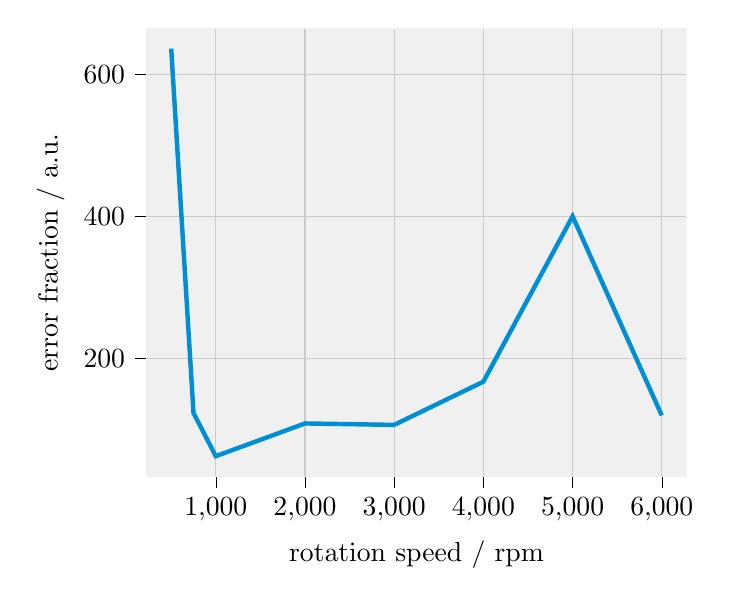
\begin{tikzpicture}

\definecolor{dodgerblue0143213}{RGB}{0,143,213}
\definecolor{lightgray203}{RGB}{203,203,203}
\definecolor{whitesmoke240}{RGB}{240,240,240}

\begin{axis}[
axis background/.style={fill=whitesmoke240},
axis line style={whitesmoke240},
tick align=outside,
tick pos=left,
x grid style={lightgray203},
xlabel={rotation speed / rpm},
xmajorgrids,
xmin=225, xmax=6275,
xtick style={color=black},
y grid style={lightgray203},
ylabel={error fraction / a.u.},
ymajorgrids,
ymin=33.6365966556009, ymax=665.114384574023,
ytick style={color=black}
]
\addplot [ultra thick, dodgerblue0143213]
table {%
500 636.410848759549
750 123.173641739447
1000 62.3401324700746
2000 108.439051217311
3000 106.413349856621
4000 167.259174437374
5000 400.186003381121
6000 119.684876758419
};
\end{axis}

\end{tikzpicture}

%     \caption{The standard deviation divided by the fit error}
%     \label{fig:errorFrac}

% \end{figure}

\begin{figure}[h]
    \centering
    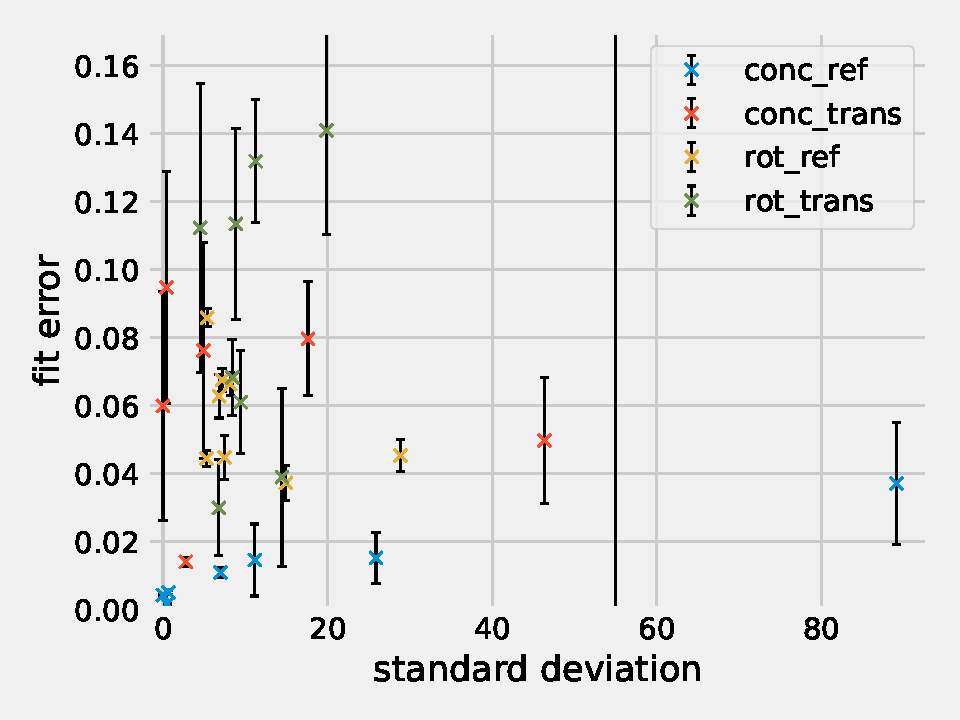
\includegraphics[width = 10cm]{Programmien/FitFehlergegenstd/FitFehlergegenStd.pdf}
    \caption{Fit error plotted against the standard deviation of the film thickness.}
    \label{fig:FitFehlergegenStd}
\end{figure}


Furthermore, we determined the mean values and the standard deviation for every measurement on the same sample. To verify whether the is a 
linear connection between the two errors we plot the fraction of those two quantities as depicted in Figure \ref{fig:errorFrac}. We were not able to find a connection.
In our interpretation the deviations are not linked since they do not have the same origin. The standard deviation in film thickness is 
not an error of measurement but a real local variation of the film thickness. The fit error in contrast is a real error. Therefore those two quantities do not seem to be linked. When
comparing the two quantities graphically as shown in Figure \ref{fig:FitFehlergegenStd}, we do not see any significant correlation.



To investigate this heterogeneity

\begin{equation}
    h = \frac{< d >}{std(d)}
\end{equation}

in more detail, we plot it against the thickness of the layer. As can be noted in Figure \ref{fig:thickheter}, the heterogeneity
increases for lower film thickness. The last point at \SI{0}{\nano\meter} has not to be taken into account since at this point the heterogeneity loses its meaning as all measurement 
return as thickness \SI{0}{\nano\meter}.

\begin{figure}[h]
    \centering
    % This file was created with tikzplotlib v0.10.1.
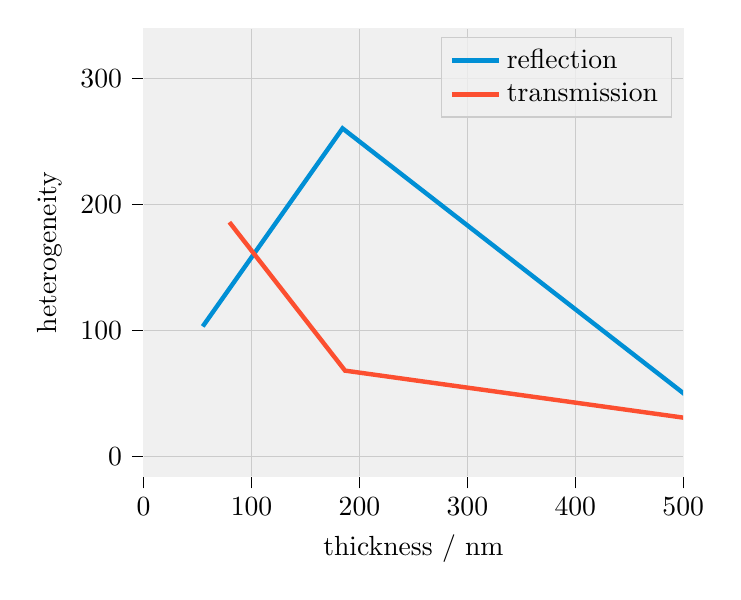
\begin{tikzpicture}

\definecolor{dodgerblue0143213}{RGB}{0,143,213}
\definecolor{lightgray203}{RGB}{203,203,203}
\definecolor{lightgray204}{RGB}{204,204,204}
\definecolor{tomato2527948}{RGB}{252,79,48}
\definecolor{whitesmoke240}{RGB}{240,240,240}

\begin{axis}[
axis background/.style={fill=whitesmoke240},
axis line style={whitesmoke240},
legend cell align={left},
legend style={fill opacity=0.8, draw opacity=1, text opacity=1, draw=lightgray204, fill=whitesmoke240},
tick align=outside,
tick pos=left,
x grid style={lightgray203},
xlabel={thickness / nm},
xmajorgrids,
xmin=0, xmax=500,
xtick style={color=black},
y grid style={lightgray203},
ylabel={heterogeneity},
ymajorgrids,
ymin=-16.1709065832112, ymax=339.589038247436,
ytick style={color=black}
]
\addplot [ultra thick, dodgerblue0143213]
table {%
54.8 102.951273454399
184.333333333333 260.109320108062
506.916666666667 45.4580969214582
1608.61666666667 230.901253116566
2390.2 92.3486037681464
3603.6 40.4234374272009
};
\addlegendentry{reflection}
\addplot [ultra thick, tomato2527948]
table {%
79.5 185.671998182523
186.633333333333 67.8828757163584
512.55 29.0913787966606
1594.4 323.418131664225
2433.08333333333 52.4743060151849
3483.85 63.3585514325261
};
\addlegendentry{transmission}
\end{axis}

\end{tikzpicture}

    \caption{Heterogeneity $h$ against film thickness.}
    \label{fig:thickheter}
\end{figure}

% \begin{figure}[h]
%     \centering
%     \begin{subfigure}[b]{0.70\textwidth}
%         \centering
%         % This file was created with tikzplotlib v0.10.1.
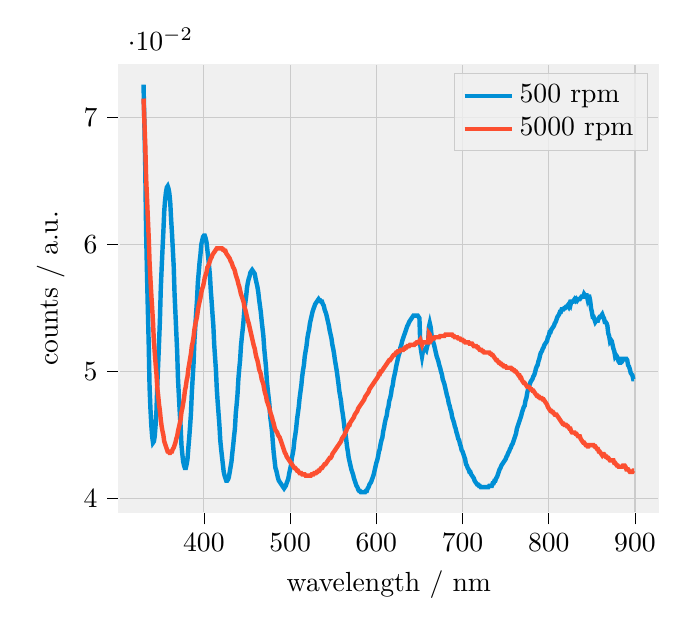
\begin{tikzpicture}

\definecolor{dodgerblue0143213}{RGB}{0,143,213}
\definecolor{lightgray203}{RGB}{203,203,203}
\definecolor{lightgray204}{RGB}{204,204,204}
\definecolor{tomato2527948}{RGB}{252,79,48}
\definecolor{whitesmoke240}{RGB}{240,240,240}

\begin{axis}[
axis background/.style={fill=whitesmoke240},
axis line style={whitesmoke240},
legend cell align={left},
legend style={fill opacity=0.8, draw opacity=1, text opacity=1, draw=lightgray204, fill=whitesmoke240},
tick align=outside,
tick pos=left,
x grid style={lightgray203},
xlabel={wavelength / nm},
xmajorgrids,
xmin=301.55, xmax=927.45,
xtick style={color=black},
y grid style={lightgray203},
ylabel={counts / a.u.},
ymajorgrids,
ymin=0.038895, ymax=0.074205,
ytick style={color=black}
]
\addplot [ultra thick, dodgerblue0143213]
table {%
330 0.0726
331 0.0695
332 0.0661
333 0.061
334 0.0578
335 0.0549
336 0.0522
337 0.0488
338 0.0471
339 0.0458
340 0.0449
341 0.0444
342 0.0445
343 0.0449
344 0.0458
345 0.0469
346 0.049
347 0.0506
348 0.0523
349 0.054
350 0.0565
351 0.0581
352 0.0596
353 0.061
354 0.0626
355 0.0635
356 0.0641
357 0.0645
358 0.0646
359 0.0644
360 0.064
361 0.0633
362 0.062
363 0.0609
364 0.0596
365 0.0583
366 0.0561
367 0.0546
368 0.0531
369 0.0516
370 0.0494
371 0.0481
372 0.0468
373 0.0457
374 0.0442
375 0.0435
376 0.0429
377 0.0426
378 0.0424
379 0.0424
380 0.0427
381 0.0431
382 0.044
383 0.0448
384 0.0457
385 0.0467
386 0.0483
387 0.0495
388 0.0506
389 0.0524
390 0.0535
391 0.0546
392 0.0556
393 0.057
394 0.0578
395 0.0586
396 0.0592
397 0.06
398 0.0603
399 0.0606
400 0.0607
401 0.0607
402 0.0605
403 0.0602
404 0.0596
405 0.059
406 0.0583
407 0.0576
408 0.0564
409 0.0555
410 0.0545
411 0.0536
412 0.0521
413 0.0511
414 0.0501
415 0.0486
416 0.0476
417 0.0467
418 0.0458
419 0.0446
420 0.0439
421 0.0433
422 0.0427
423 0.0421
424 0.0418
425 0.0416
426 0.0414
427 0.0414
428 0.0415
429 0.0417
430 0.0421
431 0.0425
432 0.0429
433 0.0436
434 0.0442
435 0.0449
436 0.0455
437 0.0467
438 0.0474
439 0.0482
440 0.0494
441 0.0502
442 0.0509
443 0.052
444 0.0527
445 0.0533
446 0.054
447 0.0549
448 0.0554
449 0.0559
450 0.0566
451 0.057
452 0.0573
453 0.0575
454 0.0578
455 0.0579
456 0.058
457 0.0579
458 0.0578
459 0.0577
460 0.0573
461 0.057
462 0.0567
463 0.0563
464 0.0557
465 0.0552
466 0.0547
467 0.054
468 0.0534
469 0.0528
470 0.0518
471 0.0511
472 0.0504
473 0.0493
474 0.0486
475 0.048
476 0.0474
477 0.0464
478 0.0459
479 0.0453
480 0.0444
481 0.0436
482 0.043
483 0.0424
484 0.0422
485 0.0419
486 0.0416
487 0.0414
488 0.0413
489 0.0412
490 0.0411
491 0.041
492 0.0409
493 0.0408
494 0.0409
495 0.041
496 0.0412
497 0.0414
498 0.0416
499 0.042
500 0.0423
501 0.0426
502 0.0432
503 0.0435
504 0.0439
505 0.0446
506 0.045
507 0.0455
508 0.0462
509 0.0467
510 0.0472
511 0.0479
512 0.0484
513 0.0489
514 0.0496
515 0.0501
516 0.0505
517 0.0512
518 0.0516
519 0.052
520 0.0526
521 0.053
522 0.0533
523 0.0538
524 0.0541
525 0.0544
526 0.0547
527 0.0549
528 0.0551
529 0.0553
530 0.0554
531 0.0555
532 0.0556
533 0.0557
534 0.0556
535 0.0556
536 0.0555
537 0.0555
538 0.0553
539 0.0552
540 0.0549
541 0.0547
542 0.0545
543 0.0542
544 0.0539
545 0.0536
546 0.0532
547 0.0529
548 0.0526
549 0.0521
550 0.0518
551 0.0514
552 0.0509
553 0.0505
554 0.0501
555 0.0496
556 0.0491
557 0.0485
558 0.0481
559 0.0477
560 0.0471
561 0.0467
562 0.0462
563 0.0456
564 0.0452
565 0.0447
566 0.0441
567 0.0437
568 0.0432
569 0.0429
570 0.0426
571 0.0423
572 0.0421
573 0.0419
574 0.0416
575 0.0414
576 0.0412
577 0.041
578 0.0409
579 0.0407
580 0.0406
581 0.0406
582 0.0405
583 0.0405
584 0.0405
585 0.0405
586 0.0405
587 0.0405
588 0.0406
589 0.0406
590 0.0408
591 0.0409
592 0.0411
593 0.0412
594 0.0413
595 0.0415
596 0.0417
597 0.0419
598 0.0422
599 0.0425
600 0.0428
601 0.043
602 0.0433
603 0.0437
604 0.0439
605 0.0443
606 0.0446
607 0.0448
608 0.0453
609 0.0456
610 0.046
611 0.0463
612 0.0465
613 0.047
614 0.0472
615 0.0477
616 0.0479
617 0.0482
618 0.0487
619 0.0489
620 0.0494
621 0.0497
622 0.05
623 0.0504
624 0.0507
625 0.051
626 0.0513
627 0.0515
628 0.0519
629 0.0521
630 0.0524
631 0.0526
632 0.0528
633 0.053
634 0.0532
635 0.0534
636 0.0536
637 0.0537
638 0.0539
639 0.054
640 0.0541
641 0.0542
642 0.0543
643 0.0544
644 0.0544
645 0.0544
646 0.0544
647 0.0544
648 0.0544
649 0.0543
650 0.0542
651 0.0521
652 0.0516
653 0.0512
654 0.0516
655 0.0517
656 0.0517
657 0.0518
658 0.0517
659 0.052
660 0.0522
661 0.0535
662 0.0538
663 0.0535
664 0.0529
665 0.0526
666 0.0523
667 0.0521
668 0.0518
669 0.0515
670 0.0512
671 0.051
672 0.0508
673 0.0505
674 0.0503
675 0.05
676 0.0498
677 0.0494
678 0.0492
679 0.049
680 0.0487
681 0.0484
682 0.0481
683 0.0479
684 0.0475
685 0.0473
686 0.047
687 0.0468
688 0.0464
689 0.0462
690 0.046
691 0.0457
692 0.0455
693 0.0452
694 0.045
695 0.0447
696 0.0446
697 0.0443
698 0.0441
699 0.0438
700 0.0437
701 0.0435
702 0.0433
703 0.0431
704 0.0427
705 0.0426
706 0.0424
707 0.0423
708 0.0421
709 0.0421
710 0.0419
711 0.0418
712 0.0417
713 0.0416
714 0.0414
715 0.0413
716 0.0412
717 0.0411
718 0.0411
719 0.041
720 0.041
721 0.0409
722 0.0409
723 0.0409
724 0.0409
725 0.0409
726 0.0409
727 0.0409
728 0.0409
729 0.0409
730 0.0409
731 0.041
732 0.041
733 0.041
734 0.041
735 0.0412
736 0.0412
737 0.0414
738 0.0414
739 0.0416
740 0.0417
741 0.0419
742 0.0421
743 0.0423
744 0.0424
745 0.0426
746 0.0427
747 0.0428
748 0.0429
749 0.043
750 0.0431
751 0.0433
752 0.0434
753 0.0436
754 0.0437
755 0.0439
756 0.044
757 0.0442
758 0.0443
759 0.0445
760 0.0447
761 0.0449
762 0.0451
763 0.0455
764 0.0457
765 0.0459
766 0.0461
767 0.0463
768 0.0465
769 0.0468
770 0.047
771 0.0472
772 0.0473
773 0.0477
774 0.0479
775 0.0483
776 0.0486
777 0.0488
778 0.049
779 0.0492
780 0.0493
781 0.0494
782 0.0496
783 0.0497
784 0.0499
785 0.0502
786 0.0504
787 0.0505
788 0.0508
789 0.051
790 0.0513
791 0.0515
792 0.0516
793 0.0518
794 0.0519
795 0.0521
796 0.0522
797 0.0523
798 0.0524
799 0.0527
800 0.0528
801 0.0531
802 0.0531
803 0.0533
804 0.0534
805 0.0535
806 0.0536
807 0.0538
808 0.0539
809 0.0541
810 0.0543
811 0.0544
812 0.0545
813 0.0547
814 0.0547
815 0.0549
816 0.0549
817 0.0549
818 0.055
819 0.055
820 0.0551
821 0.0551
822 0.0552
823 0.0551
824 0.0553
825 0.0552
826 0.0555
827 0.0555
828 0.0555
829 0.0556
830 0.0557
831 0.0556
832 0.0557
833 0.0556
834 0.0557
835 0.0557
836 0.0557
837 0.0558
838 0.0559
839 0.0559
840 0.0559
841 0.0561
842 0.056
843 0.056
844 0.056
845 0.0557
846 0.0559
847 0.0559
848 0.0556
849 0.055
850 0.0547
851 0.0543
852 0.0543
853 0.0541
854 0.0539
855 0.054
856 0.054
857 0.054
858 0.0542
859 0.0543
860 0.0543
861 0.0544
862 0.0545
863 0.0543
864 0.0542
865 0.0539
866 0.0539
867 0.0538
868 0.0536
869 0.053
870 0.0528
871 0.0524
872 0.0525
873 0.0524
874 0.0521
875 0.0518
876 0.0516
877 0.0512
878 0.0513
879 0.0512
880 0.051
881 0.0508
882 0.0507
883 0.0507
884 0.051
885 0.051
886 0.0509
887 0.051
888 0.051
889 0.051
890 0.051
891 0.0509
892 0.0505
893 0.0504
894 0.0502
895 0.0499
896 0.0498
897 0.0497
898 0.0494
899 0.0494
};
\addlegendentry{500 rpm}
\addplot [ultra thick, tomato2527948]
table {%
330 0.0715
331 0.0697
332 0.0679
333 0.0653
334 0.0637
335 0.0621
336 0.0606
337 0.0586
338 0.0573
339 0.0561
340 0.055
341 0.0539
342 0.0524
343 0.0515
344 0.0506
345 0.0498
346 0.0487
347 0.0481
348 0.0474
349 0.0469
350 0.0462
351 0.0457
352 0.0453
353 0.045
354 0.0445
355 0.0443
356 0.0441
357 0.0439
358 0.0437
359 0.0437
360 0.0436
361 0.0436
362 0.0437
363 0.0437
364 0.0439
365 0.044
366 0.0442
367 0.0444
368 0.0447
369 0.0449
370 0.0453
371 0.0456
372 0.0459
373 0.0462
374 0.0468
375 0.0471
376 0.0475
377 0.0479
378 0.0485
379 0.0488
380 0.0493
381 0.0496
382 0.0502
383 0.0506
384 0.051
385 0.0514
386 0.052
387 0.0523
388 0.0527
389 0.0533
390 0.0537
391 0.054
392 0.0543
393 0.0548
394 0.0552
395 0.0555
396 0.0558
397 0.0562
398 0.0565
399 0.0567
400 0.057
401 0.0574
402 0.0576
403 0.0578
404 0.0582
405 0.0583
406 0.0585
407 0.0587
408 0.0589
409 0.059
410 0.0592
411 0.0593
412 0.0594
413 0.0595
414 0.0596
415 0.0597
416 0.0597
417 0.0597
418 0.0597
419 0.0597
420 0.0597
421 0.0597
422 0.0596
423 0.0596
424 0.0595
425 0.0595
426 0.0593
427 0.0592
428 0.0591
429 0.059
430 0.0589
431 0.0587
432 0.0586
433 0.0584
434 0.0582
435 0.0581
436 0.0579
437 0.0576
438 0.0574
439 0.0572
440 0.0569
441 0.0567
442 0.0564
443 0.0561
444 0.0559
445 0.0557
446 0.0555
447 0.0551
448 0.0549
449 0.0546
450 0.0543
451 0.054
452 0.0538
453 0.0535
454 0.0532
455 0.0529
456 0.0526
457 0.0523
458 0.052
459 0.0518
460 0.0514
461 0.0511
462 0.0509
463 0.0506
464 0.0502
465 0.05
466 0.0498
467 0.0494
468 0.0492
469 0.049
470 0.0486
471 0.0483
472 0.0481
473 0.0477
474 0.0475
475 0.0473
476 0.0471
477 0.0468
478 0.0466
479 0.0464
480 0.0461
481 0.0459
482 0.0456
483 0.0454
484 0.0453
485 0.0452
486 0.045
487 0.0449
488 0.0448
489 0.0446
490 0.0444
491 0.0442
492 0.044
493 0.0438
494 0.0436
495 0.0435
496 0.0433
497 0.0432
498 0.0431
499 0.043
500 0.0429
501 0.0428
502 0.0427
503 0.0426
504 0.0425
505 0.0424
506 0.0424
507 0.0423
508 0.0422
509 0.0422
510 0.0421
511 0.042
512 0.042
513 0.042
514 0.0419
515 0.0419
516 0.0419
517 0.0419
518 0.0418
519 0.0418
520 0.0418
521 0.0418
522 0.0418
523 0.0418
524 0.0418
525 0.0419
526 0.0419
527 0.0419
528 0.042
529 0.042
530 0.042
531 0.0421
532 0.0421
533 0.0422
534 0.0422
535 0.0423
536 0.0424
537 0.0424
538 0.0425
539 0.0426
540 0.0427
541 0.0427
542 0.0428
543 0.0429
544 0.043
545 0.0431
546 0.0432
547 0.0432
548 0.0433
549 0.0435
550 0.0436
551 0.0437
552 0.0438
553 0.0439
554 0.044
555 0.0441
556 0.0442
557 0.0443
558 0.0444
559 0.0445
560 0.0447
561 0.0448
562 0.0449
563 0.045
564 0.0452
565 0.0453
566 0.0455
567 0.0456
568 0.0458
569 0.0458
570 0.046
571 0.0461
572 0.0462
573 0.0463
574 0.0464
575 0.0466
576 0.0467
577 0.0468
578 0.0469
579 0.0471
580 0.0472
581 0.0473
582 0.0474
583 0.0475
584 0.0476
585 0.0477
586 0.0478
587 0.048
588 0.0481
589 0.0482
590 0.0483
591 0.0484
592 0.0486
593 0.0487
594 0.0488
595 0.0489
596 0.049
597 0.0491
598 0.0492
599 0.0493
600 0.0494
601 0.0495
602 0.0496
603 0.0498
604 0.0498
605 0.05
606 0.05
607 0.0501
608 0.0502
609 0.0503
610 0.0504
611 0.0505
612 0.0506
613 0.0507
614 0.0508
615 0.0509
616 0.0509
617 0.051
618 0.0511
619 0.0512
620 0.0513
621 0.0513
622 0.0514
623 0.0515
624 0.0515
625 0.0516
626 0.0516
627 0.0516
628 0.0517
629 0.0517
630 0.0517
631 0.0517
632 0.0518
633 0.0518
634 0.0519
635 0.0519
636 0.052
637 0.052
638 0.052
639 0.0521
640 0.0521
641 0.0521
642 0.0521
643 0.0521
644 0.0521
645 0.0522
646 0.0522
647 0.0523
648 0.0523
649 0.0523
650 0.0524
651 0.0525
652 0.0523
653 0.0521
654 0.0523
655 0.0523
656 0.0523
657 0.0523
658 0.0523
659 0.0523
660 0.0523
661 0.053
662 0.0529
663 0.0527
664 0.0525
665 0.0526
666 0.0526
667 0.0526
668 0.0527
669 0.0527
670 0.0527
671 0.0527
672 0.0527
673 0.0527
674 0.0528
675 0.0528
676 0.0528
677 0.0528
678 0.0528
679 0.0528
680 0.0529
681 0.0529
682 0.0529
683 0.0529
684 0.0529
685 0.0529
686 0.0529
687 0.0529
688 0.0529
689 0.0528
690 0.0528
691 0.0527
692 0.0527
693 0.0527
694 0.0527
695 0.0526
696 0.0526
697 0.0526
698 0.0525
699 0.0525
700 0.0525
701 0.0524
702 0.0524
703 0.0523
704 0.0523
705 0.0523
706 0.0523
707 0.0523
708 0.0522
709 0.0522
710 0.0522
711 0.0522
712 0.0521
713 0.052
714 0.052
715 0.052
716 0.052
717 0.0519
718 0.0519
719 0.0518
720 0.0517
721 0.0517
722 0.0517
723 0.0516
724 0.0516
725 0.0515
726 0.0515
727 0.0515
728 0.0515
729 0.0515
730 0.0515
731 0.0515
732 0.0514
733 0.0514
734 0.0513
735 0.0513
736 0.0512
737 0.0511
738 0.051
739 0.0509
740 0.0509
741 0.0508
742 0.0507
743 0.0507
744 0.0506
745 0.0506
746 0.0505
747 0.0505
748 0.0504
749 0.0504
750 0.0504
751 0.0503
752 0.0503
753 0.0503
754 0.0503
755 0.0503
756 0.0503
757 0.0502
758 0.0502
759 0.0501
760 0.0501
761 0.05
762 0.05
763 0.0499
764 0.0498
765 0.0497
766 0.0497
767 0.0495
768 0.0495
769 0.0493
770 0.0492
771 0.0491
772 0.0491
773 0.049
774 0.0489
775 0.0488
776 0.0488
777 0.0488
778 0.0487
779 0.0486
780 0.0486
781 0.0485
782 0.0485
783 0.0484
784 0.0483
785 0.0482
786 0.0481
787 0.0481
788 0.048
789 0.048
790 0.0479
791 0.0479
792 0.0479
793 0.0478
794 0.0478
795 0.0477
796 0.0476
797 0.0475
798 0.0474
799 0.0472
800 0.0471
801 0.047
802 0.0469
803 0.0469
804 0.0468
805 0.0468
806 0.0467
807 0.0466
808 0.0466
809 0.0466
810 0.0465
811 0.0464
812 0.0463
813 0.0462
814 0.0461
815 0.046
816 0.0459
817 0.0459
818 0.0458
819 0.0458
820 0.0458
821 0.0457
822 0.0457
823 0.0456
824 0.0455
825 0.0455
826 0.0453
827 0.0452
828 0.0452
829 0.0452
830 0.0452
831 0.0451
832 0.0451
833 0.045
834 0.0449
835 0.0449
836 0.0449
837 0.0447
838 0.0446
839 0.0445
840 0.0444
841 0.0444
842 0.0443
843 0.0442
844 0.0442
845 0.0441
846 0.0441
847 0.0442
848 0.0442
849 0.0442
850 0.0442
851 0.0442
852 0.0442
853 0.0441
854 0.0441
855 0.044
856 0.0439
857 0.0439
858 0.0437
859 0.0437
860 0.0436
861 0.0435
862 0.0434
863 0.0435
864 0.0435
865 0.0434
866 0.0433
867 0.0433
868 0.0432
869 0.0432
870 0.0431
871 0.043
872 0.043
873 0.043
874 0.043
875 0.043
876 0.0428
877 0.0428
878 0.0427
879 0.0426
880 0.0426
881 0.0425
882 0.0425
883 0.0425
884 0.0425
885 0.0425
886 0.0426
887 0.0426
888 0.0426
889 0.0425
890 0.0423
891 0.0423
892 0.0423
893 0.0422
894 0.0421
895 0.0421
896 0.0421
897 0.0421
898 0.0422
899 0.0422
};
\addlegendentry{5000 rpm}
\end{axis}

\end{tikzpicture}

%         \caption{$Reflectance$}
%         \label{fig:y equals x}
%     \end{subfigure}  
    

%     \begin{subfigure}[b]{0.70\textwidth}
%         \centering
%         % This file was created with tikzplotlib v0.10.1.
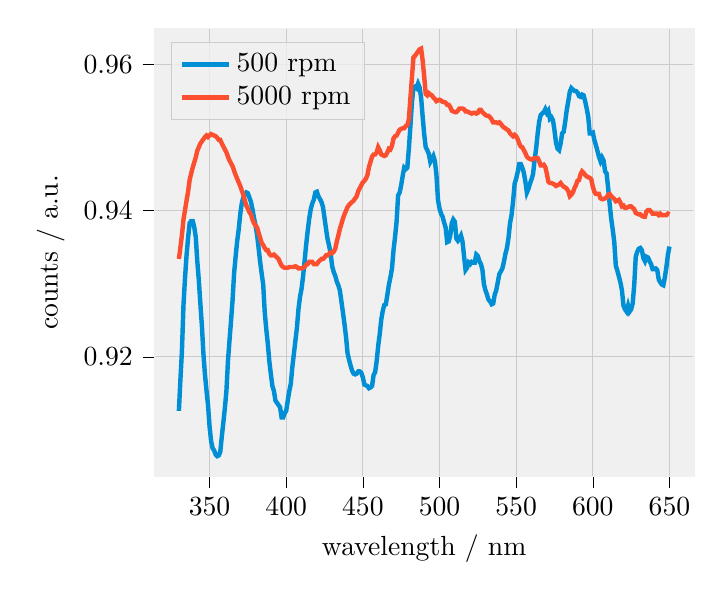
\begin{tikzpicture}

\definecolor{dodgerblue0143213}{RGB}{0,143,213}
\definecolor{lightgray203}{RGB}{203,203,203}
\definecolor{lightgray204}{RGB}{204,204,204}
\definecolor{tomato2527948}{RGB}{252,79,48}
\definecolor{whitesmoke240}{RGB}{240,240,240}

\begin{axis}[
axis background/.style={fill=whitesmoke240},
axis line style={whitesmoke240},
legend cell align={left},
legend style={
  fill opacity=0.8,
  draw opacity=1,
  text opacity=1,
  at={(0.03,0.97)},
  anchor=north west,
  draw=lightgray204,
  fill=whitesmoke240
},
tick align=outside,
tick pos=left,
x grid style={lightgray203},
xlabel={wavelength / nm},
xmajorgrids,
xmin=314, xmax=666,
xtick style={color=black},
y grid style={lightgray203},
ylabel={counts / a.u.},
ymajorgrids,
ymin=0.90361, ymax=0.96499,
ytick style={color=black}
]
\addplot [ultra thick, dodgerblue0143213]
table {%
330 0.9126
331 0.9169
332 0.9209
333 0.9271
334 0.9308
335 0.9339
336 0.9363
337 0.9383
338 0.9386
339 0.9386
340 0.9378
341 0.9364
342 0.9331
343 0.9305
344 0.9273
345 0.9243
346 0.9204
347 0.9176
348 0.9154
349 0.9134
350 0.9105
351 0.9085
352 0.9075
353 0.9072
354 0.9066
355 0.9064
356 0.9065
357 0.907
358 0.9091
359 0.911
360 0.913
361 0.9153
362 0.9194
363 0.9222
364 0.9249
365 0.9277
366 0.9314
367 0.9337
368 0.9358
369 0.9374
370 0.9395
371 0.941
372 0.9418
373 0.9422
374 0.9425
375 0.9424
376 0.9418
377 0.9412
378 0.9402
379 0.939
380 0.938
381 0.9367
382 0.9349
383 0.933
384 0.9314
385 0.9299
386 0.9261
387 0.9238
388 0.9218
389 0.9194
390 0.9176
391 0.916
392 0.9153
393 0.914
394 0.9137
395 0.9134
396 0.9131
397 0.9117
398 0.9117
399 0.9123
400 0.9126
401 0.914
402 0.9153
403 0.9163
404 0.9186
405 0.9204
406 0.9222
407 0.924
408 0.9265
409 0.9282
410 0.9293
411 0.931
412 0.9331
413 0.9353
414 0.9372
415 0.9389
416 0.9402
417 0.941
418 0.9415
419 0.9425
420 0.9426
421 0.942
422 0.9416
423 0.9412
424 0.9405
425 0.939
426 0.9375
427 0.9361
428 0.9352
429 0.9341
430 0.9324
431 0.9316
432 0.9311
433 0.9303
434 0.9298
435 0.9291
436 0.9276
437 0.9261
438 0.9245
439 0.9228
440 0.9205
441 0.9196
442 0.9188
443 0.9181
444 0.9177
445 0.9176
446 0.9177
447 0.918
448 0.918
449 0.9178
450 0.9172
451 0.9162
452 0.9161
453 0.916
454 0.9157
455 0.9158
456 0.916
457 0.9175
458 0.9179
459 0.9194
460 0.9215
461 0.9231
462 0.9251
463 0.9263
464 0.9271
465 0.9272
466 0.9285
467 0.9299
468 0.9309
469 0.9321
470 0.9346
471 0.9364
472 0.9385
473 0.9421
474 0.9425
475 0.9435
476 0.9448
477 0.9459
478 0.9457
479 0.9459
480 0.9485
481 0.9515
482 0.9548
483 0.9569
484 0.957
485 0.9568
486 0.9574
487 0.9569
488 0.9555
489 0.9529
490 0.9505
491 0.9487
492 0.9483
493 0.9478
494 0.9467
495 0.9471
496 0.9475
497 0.9468
498 0.9449
499 0.9415
500 0.9403
501 0.9396
502 0.9392
503 0.9384
504 0.9377
505 0.9357
506 0.9358
507 0.9366
508 0.9383
509 0.9388
510 0.9385
511 0.9362
512 0.9359
513 0.9362
514 0.9366
515 0.9358
516 0.9338
517 0.9319
518 0.9322
519 0.9329
520 0.9327
521 0.933
522 0.9329
523 0.9329
524 0.934
525 0.9338
526 0.9331
527 0.9327
528 0.9319
529 0.9299
530 0.9291
531 0.9285
532 0.9278
533 0.9276
534 0.9272
535 0.9273
536 0.9285
537 0.9291
538 0.9302
539 0.9313
540 0.9317
541 0.9321
542 0.933
543 0.9341
544 0.9349
545 0.9363
546 0.9383
547 0.9394
548 0.9413
549 0.9437
550 0.9444
551 0.9453
552 0.9464
553 0.9464
554 0.9459
555 0.9452
556 0.944
557 0.9425
558 0.943
559 0.9437
560 0.9443
561 0.945
562 0.9469
563 0.9485
564 0.9505
565 0.9522
566 0.9531
567 0.9533
568 0.9535
569 0.9539
570 0.9534
571 0.9537
572 0.9526
573 0.9528
574 0.9524
575 0.951
576 0.9493
577 0.9485
578 0.9483
579 0.9492
580 0.9506
581 0.9508
582 0.9522
583 0.9538
584 0.955
585 0.9563
586 0.9568
587 0.9566
588 0.9564
589 0.9564
590 0.9562
591 0.9557
592 0.9556
593 0.9559
594 0.9558
595 0.955
596 0.954
597 0.9529
598 0.9506
599 0.9506
600 0.9507
601 0.9497
602 0.949
603 0.9482
604 0.9474
605 0.9468
606 0.9473
607 0.9469
608 0.9454
609 0.9451
610 0.9431
611 0.9409
612 0.9389
613 0.9374
614 0.9357
615 0.9325
616 0.9318
617 0.931
618 0.9302
619 0.9291
620 0.927
621 0.9265
622 0.9262
623 0.927
624 0.9262
625 0.9265
626 0.9273
627 0.9298
628 0.9337
629 0.9344
630 0.9348
631 0.9349
632 0.9346
633 0.9335
634 0.9331
635 0.9337
636 0.9336
637 0.9331
638 0.9327
639 0.932
640 0.932
641 0.9321
642 0.9319
643 0.9306
644 0.9302
645 0.9299
646 0.9298
647 0.9309
648 0.9323
649 0.934
650 0.9351
};
\addlegendentry{500 rpm}
\addplot [ultra thick, tomato2527948]
table {%
330 0.9334
331 0.935
332 0.9367
333 0.9388
334 0.9401
335 0.9414
336 0.9426
337 0.9442
338 0.9451
339 0.9459
340 0.9466
341 0.9473
342 0.9482
343 0.9487
344 0.9492
345 0.9495
346 0.9498
347 0.9501
348 0.9503
349 0.9501
350 0.9503
351 0.9505
352 0.9504
353 0.9503
354 0.9502
355 0.95
356 0.9497
357 0.9497
358 0.9492
359 0.9488
360 0.9484
361 0.948
362 0.9474
363 0.9469
364 0.9465
365 0.9461
366 0.9455
367 0.9449
368 0.9444
369 0.9439
370 0.9434
371 0.9428
372 0.9422
373 0.9414
374 0.9407
375 0.9403
376 0.9398
377 0.9395
378 0.9388
379 0.9383
380 0.938
381 0.9377
382 0.937
383 0.9363
384 0.9356
385 0.9353
386 0.9349
387 0.9346
388 0.9346
389 0.9341
390 0.9339
391 0.9339
392 0.934
393 0.9338
394 0.9336
395 0.9334
396 0.9329
397 0.9325
398 0.9323
399 0.9322
400 0.9322
401 0.9322
402 0.9323
403 0.9323
404 0.9323
405 0.9323
406 0.9324
407 0.9323
408 0.9321
409 0.9321
410 0.9321
411 0.9322
412 0.9323
413 0.9326
414 0.9327
415 0.933
416 0.933
417 0.933
418 0.9327
419 0.9327
420 0.9327
421 0.933
422 0.9332
423 0.9334
424 0.9334
425 0.9336
426 0.9339
427 0.9339
428 0.9341
429 0.9343
430 0.9342
431 0.9344
432 0.9348
433 0.9358
434 0.9366
435 0.9375
436 0.9382
437 0.9389
438 0.9395
439 0.94
440 0.9405
441 0.9408
442 0.941
443 0.9412
444 0.9414
445 0.9417
446 0.942
447 0.9427
448 0.9431
449 0.9435
450 0.9439
451 0.9441
452 0.9444
453 0.9449
454 0.946
455 0.9467
456 0.9474
457 0.9477
458 0.9477
459 0.948
460 0.9487
461 0.9483
462 0.9477
463 0.9476
464 0.9475
465 0.9476
466 0.948
467 0.9485
468 0.9484
469 0.9489
470 0.9499
471 0.9502
472 0.9503
473 0.9507
474 0.9511
475 0.9512
476 0.9513
477 0.9513
478 0.9516
479 0.9517
480 0.9525
481 0.9554
482 0.9582
483 0.961
484 0.9612
485 0.9615
486 0.9618
487 0.9621
488 0.9622
489 0.9606
490 0.9584
491 0.956
492 0.9558
493 0.9561
494 0.9559
495 0.9558
496 0.9555
497 0.9553
498 0.955
499 0.9551
500 0.9552
501 0.9551
502 0.9549
503 0.9549
504 0.9548
505 0.9545
506 0.9545
507 0.9542
508 0.9537
509 0.9536
510 0.9535
511 0.9535
512 0.9537
513 0.954
514 0.954
515 0.954
516 0.9539
517 0.9536
518 0.9536
519 0.9535
520 0.9534
521 0.9533
522 0.9534
523 0.9534
524 0.9533
525 0.9534
526 0.9538
527 0.9538
528 0.9535
529 0.9533
530 0.9531
531 0.953
532 0.953
533 0.9528
534 0.9525
535 0.9521
536 0.9521
537 0.9521
538 0.952
539 0.9521
540 0.9519
541 0.9516
542 0.9514
543 0.9513
544 0.9511
545 0.951
546 0.9506
547 0.9504
548 0.9502
549 0.9504
550 0.9502
551 0.9498
552 0.9492
553 0.9488
554 0.9487
555 0.9483
556 0.9479
557 0.9474
558 0.9472
559 0.9471
560 0.947
561 0.9471
562 0.9472
563 0.9472
564 0.9472
565 0.9468
566 0.9462
567 0.9462
568 0.9463
569 0.946
570 0.9451
571 0.944
572 0.9438
573 0.9438
574 0.9437
575 0.9436
576 0.9434
577 0.9435
578 0.9436
579 0.9438
580 0.9435
581 0.9433
582 0.9432
583 0.943
584 0.9427
585 0.942
586 0.9422
587 0.9425
588 0.9431
589 0.9435
590 0.9441
591 0.9442
592 0.945
593 0.9454
594 0.9452
595 0.9449
596 0.9447
597 0.9446
598 0.9445
599 0.9443
600 0.9433
601 0.9426
602 0.9423
603 0.9423
604 0.9423
605 0.9417
606 0.9416
607 0.9416
608 0.9417
609 0.9418
610 0.9422
611 0.9423
612 0.942
613 0.9418
614 0.9416
615 0.9413
616 0.9414
617 0.9415
618 0.9411
619 0.9406
620 0.9407
621 0.9404
622 0.9404
623 0.9405
624 0.9406
625 0.9406
626 0.9404
627 0.9402
628 0.9397
629 0.9396
630 0.9395
631 0.9395
632 0.9393
633 0.9392
634 0.9392
635 0.9399
636 0.9401
637 0.9401
638 0.9399
639 0.9396
640 0.9396
641 0.9396
642 0.9396
643 0.9394
644 0.9396
645 0.9394
646 0.9394
647 0.9394
648 0.9394
649 0.9396
650 0.9395
};
\addlegendentry{5000 rpm}
\end{axis}

\end{tikzpicture}
   
%         \caption{$Transmission$} 
%         \label{fig:three sin x}
%     \end{subfigure}

%     \caption{Spectra measured in reflectance and transmission on a thin film of PS on Glass. The films are coated with different coating speeds.}
%     \label{fig:SpecRefTrans}
% \end{figure}


% \begin{figure}[h]
%     \centering
%     \begin{subfigure}[b]{\textwidth}
%         \centering
%         %\resizebox{8cm}{6cm}{
%         % This file was created with tikzplotlib v0.10.1.
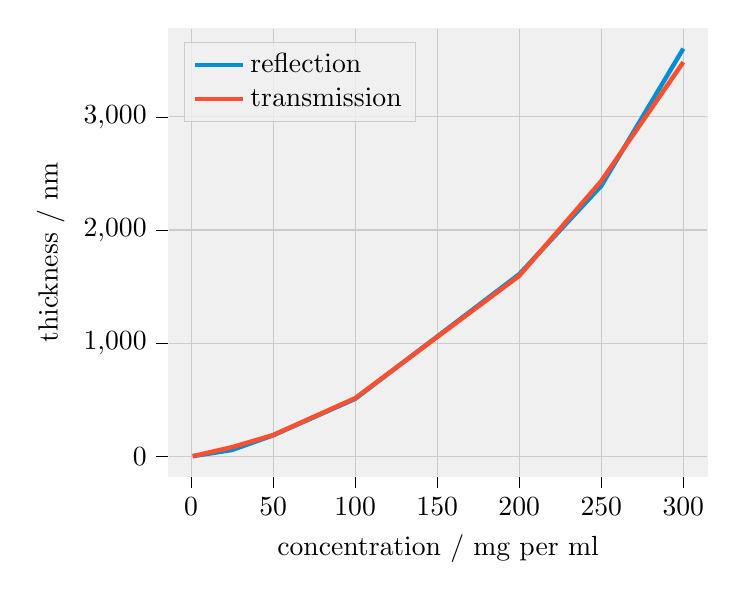
\begin{tikzpicture}

\definecolor{dodgerblue0143213}{RGB}{0,143,213}
\definecolor{lightgray203}{RGB}{203,203,203}
\definecolor{lightgray204}{RGB}{204,204,204}
\definecolor{tomato2527948}{RGB}{252,79,48}
\definecolor{whitesmoke240}{RGB}{240,240,240}

\begin{axis}[
axis background/.style={fill=whitesmoke240},
axis line style={whitesmoke240},
legend cell align={left},
legend style={
  fill opacity=0.8,
  draw opacity=1,
  text opacity=1,
  at={(0.03,0.97)},
  anchor=north west,
  draw=lightgray204,
  fill=whitesmoke240
},
tick align=outside,
tick pos=left,
x grid style={lightgray203},
xlabel={concentration / mg per ml},
xmajorgrids,
xmin=-13.95, xmax=314.95,
xtick style={color=black},
y grid style={lightgray203},
ylabel={thickness / nm},
ymajorgrids,
ymin=-180.18, ymax=3783.78,
ytick style={color=black}
]
\addplot [ultra thick, dodgerblue0143213]
table {%
1 0
25 54.8
50 184.333333333333
100 506.916666666667
200 1608.61666666667
250 2390.2
300 3603.6
};
\addlegendentry{reflection}
\addplot [ultra thick, tomato2527948]
table {%
1 0
25 79.5
50 186.633333333333
100 512.55
200 1594.4
250 2433.08333333333
300 3483.85
};
\addlegendentry{transmission}
\end{axis}

\end{tikzpicture}

%         %}
%         \caption{Thickness of the film against rotation speed during coating}
%         \label{fig:VglMethConcThick}
%     \end{subfigure}

%     \vspace{1cm}
%     \begin{subfigure}[b]{\textwidth}
%         \centering
%         % This file was created with tikzplotlib v0.10.1.
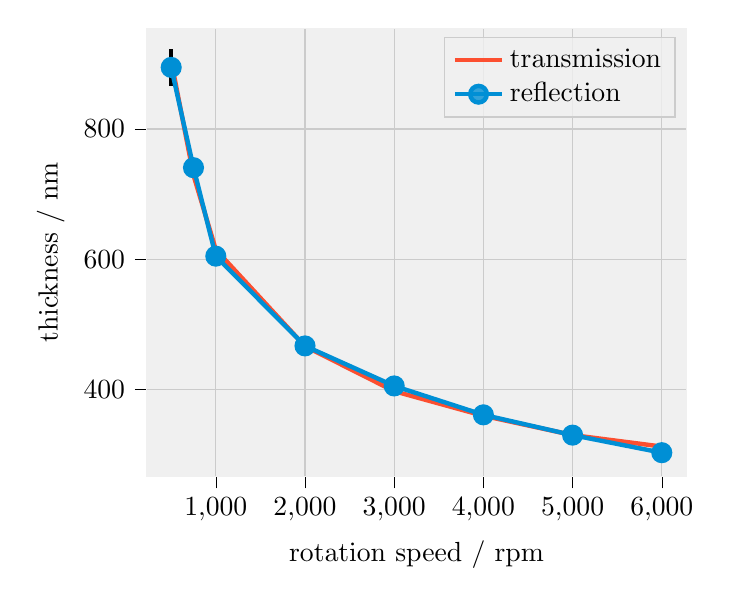
\begin{tikzpicture}

\definecolor{dodgerblue0143213}{RGB}{0,143,213}
\definecolor{lightgray203}{RGB}{203,203,203}
\definecolor{lightgray204}{RGB}{204,204,204}
\definecolor{tomato2527948}{RGB}{252,79,48}
\definecolor{whitesmoke240}{RGB}{240,240,240}

\begin{axis}[
axis background/.style={fill=whitesmoke240},
axis line style={whitesmoke240},
legend cell align={left},
legend style={fill opacity=0.8, draw opacity=1, text opacity=1, draw=lightgray204, fill=whitesmoke240},
tick align=outside,
tick pos=left,
x grid style={lightgray203},
xlabel={rotation speed / rpm},
xmajorgrids,
xmin=225, xmax=6275,
xtick style={color=black},
y grid style={lightgray203},
ylabel={thickness / nm},
ymajorgrids,
ymin=266.056164037744, ymax=954.733300161791,
ytick style={color=black}
]
\path [draw=black, ultra thick]
(axis cs:500,865.670206025666)
--(axis cs:500,923.429793974334);

\path [draw=black, ultra thick]
(axis cs:750,732.309509938563)
--(axis cs:750,748.657156728103);

\path [draw=black, ultra thick]
(axis cs:1000,599.244317659408)
--(axis cs:1000,609.955682340592);

\path [draw=black, ultra thick]
(axis cs:2000,459.903097688354)
--(axis cs:2000,473.530235644979);

\path [draw=black, ultra thick]
(axis cs:3000,398.026298881297)
--(axis cs:3000,412.407034452037);

\path [draw=black, ultra thick]
(axis cs:4000,353.366740906085)
--(axis cs:4000,368.333259093915);

\path [draw=black, ultra thick]
(axis cs:5000,314.740329019556)
--(axis cs:5000,344.593004313777);

\path [draw=black, ultra thick]
(axis cs:6000,297.359670225201)
--(axis cs:6000,308.006996441466);

\addplot [ultra thick, tomato2527948]
table {%
500 904.45
750 729.066666666667
1000 614.6
2000 466.166666666667
3000 397.166666666667
4000 359.4
5000 329.733333333333
6000 312.1
};
\addlegendentry{transmission}
\addplot [ultra thick, dodgerblue0143213, mark=*, mark size=3, mark options={solid}]
table {%
500 894.55
750 740.483333333333
1000 604.6
2000 466.716666666667
3000 405.216666666667
4000 360.85
5000 329.666666666667
6000 302.683333333333
};
\addlegendentry{reflection}
\end{axis}

\end{tikzpicture}
   
%         \caption{Thickness of the film against PS concentration of the coated solution} 
%         \label{fig:VglMethRotThick}
%     \end{subfigure}

%     \caption{Thickness output of the program \textit{NanoCalc} averaged for 6 measurement.}
%     \label{fig:thickconcrpm}
% \end{figure}
